\documentclass[11pt,preprint, authoryear]{elsarticle}

\usepackage{lmodern}
%%%% My spacing
\usepackage{setspace}
\setstretch{1.2}
\DeclareMathSizes{12}{14}{10}{10}

% Wrap around which gives all figures included the [H] command, or places it "here". This can be tedious to code in Rmarkdown.
\usepackage{float}
\let\origfigure\figure
\let\endorigfigure\endfigure
\renewenvironment{figure}[1][2] {
    \expandafter\origfigure\expandafter[H]
} {
    \endorigfigure
}

\let\origtable\table
\let\endorigtable\endtable
\renewenvironment{table}[1][2] {
    \expandafter\origtable\expandafter[H]
} {
    \endorigtable
}


\usepackage{ifxetex,ifluatex}
\usepackage{fixltx2e} % provides \textsubscript
\ifnum 0\ifxetex 1\fi\ifluatex 1\fi=0 % if pdftex
  \usepackage[T1]{fontenc}
  \usepackage[utf8]{inputenc}
\else % if luatex or xelatex
  \ifxetex
    \usepackage{mathspec}
    \usepackage{xltxtra,xunicode}
  \else
    \usepackage{fontspec}
  \fi
  \defaultfontfeatures{Mapping=tex-text,Scale=MatchLowercase}
  \newcommand{\euro}{€}
\fi

\usepackage{amssymb, amsmath, amsthm, amsfonts}

\def\bibsection{\section*{References}} %%% Make "References" appear before bibliography


\usepackage[round]{natbib}
\bibliographystyle{plainnat}

\usepackage{longtable}
\usepackage[margin=2.3cm,bottom=2cm,top=2.5cm, includefoot]{geometry}
\usepackage{fancyhdr}
\usepackage[bottom, hang, flushmargin]{footmisc}
\usepackage{graphicx}
\numberwithin{equation}{section}
\numberwithin{figure}{section}
\numberwithin{table}{section}
\setlength{\parindent}{0cm}
\setlength{\parskip}{1.3ex plus 0.5ex minus 0.3ex}
\usepackage{textcomp}
\renewcommand{\headrulewidth}{0.2pt}
\renewcommand{\footrulewidth}{0.3pt}

\usepackage{array}
\newcolumntype{x}[1]{>{\centering\arraybackslash\hspace{0pt}}p{#1}}

%%%%  Remove the "preprint submitted to" part. Don't worry about this either, it just looks better without it:
\makeatletter
\def\ps@pprintTitle{%
  \let\@oddhead\@empty
  \let\@evenhead\@empty
  \let\@oddfoot\@empty
  \let\@evenfoot\@oddfoot
}
\makeatother

 \def\tightlist{} % This allows for subbullets!

\usepackage{hyperref}
\hypersetup{breaklinks=true,
            bookmarks=true,
            colorlinks=true,
            citecolor=blue,
            urlcolor=blue,
            linkcolor=blue,
            pdfborder={0 0 0}}


% The following packages allow huxtable to work:
\usepackage{siunitx}
\usepackage{multirow}
\usepackage{hhline}
\usepackage{calc}
\usepackage{tabularx}
\usepackage{booktabs}
\usepackage{caption}


\urlstyle{same}  % don't use monospace font for urls
\setlength{\parindent}{0pt}
\setlength{\parskip}{6pt plus 2pt minus 1pt}
\setlength{\emergencystretch}{3em}  % prevent overfull lines
\setcounter{secnumdepth}{5}

%%% Use protect on footnotes to avoid problems with footnotes in titles
\let\rmarkdownfootnote\footnote%
\def\footnote{\protect\rmarkdownfootnote}
\IfFileExists{upquote.sty}{\usepackage{upquote}}{}

%%% Include extra packages specified by user
% Insert custom packages here as follows
% \usepackage{colortbl}

%%% Hard setting column skips for reports - this ensures greater consistency and control over the length settings in the document.
%% page layout
%% paragraphs
\setlength{\baselineskip}{12pt plus 0pt minus 0pt}
\setlength{\parskip}{12pt plus 0pt minus 0pt}
\setlength{\parindent}{0pt plus 0pt minus 0pt}
%% floats
\setlength{\floatsep}{12pt plus 0 pt minus 0pt}
\setlength{\textfloatsep}{20pt plus 0pt minus 0pt}
\setlength{\intextsep}{14pt plus 0pt minus 0pt}
\setlength{\dbltextfloatsep}{20pt plus 0pt minus 0pt}
\setlength{\dblfloatsep}{14pt plus 0pt minus 0pt}
%% maths
\setlength{\abovedisplayskip}{12pt plus 0pt minus 0pt}
\setlength{\belowdisplayskip}{12pt plus 0pt minus 0pt}
%% lists
\setlength{\topsep}{10pt plus 0pt minus 0pt}
\setlength{\partopsep}{3pt plus 0pt minus 0pt}
\setlength{\itemsep}{5pt plus 0pt minus 0pt}
\setlength{\labelsep}{8mm plus 0mm minus 0mm}
\setlength{\parsep}{\the\parskip}
\setlength{\listparindent}{\the\parindent}
%% verbatim
\setlength{\fboxsep}{5pt plus 0pt minus 0pt}



\begin{document}

\begin{frontmatter}  %

\title{Assessing the co-movement in emerging market equity indices: Using
Dynamic Conditional Correlations in the pre and post crisis era under
low and high global uncertainty episodes}

% Set to FALSE if wanting to remove title (for submission)




\author[Add1]{Tangeni Shatiwa}
\ead{tangenishatiwa1994@gmail.com}





\address[Add1]{Department of Economics, Stellenbosch University, South Africa}


\begin{abstract}
\small{
This paper investigates the extent of conditional volatility and
time-varying correlations in South African and 18 other emerging market
equity indices between January 2000 and November 2019. With
considerations related to the dynamics in returns and correlation being
focal drivers in the trajectory of asset pricing and hedging strategies,
the multivariate DCC-GARCH model is used to study these characteristics
extensively. Specifically, these estimates are decomposed into pre and
post global financial crisis periods in attempt to understand how the
dynamics have evolved since the crisis' onset. Furthermore, episodes of
high and low financial market volatility are characterised by
stratifying the CBOE VIX into quintiles to assess whether these episodes
intensify the correlations between equity indices. Overall, the main
findings suggest a sharp rise in these co-movements in the post-Lehman
era, as well as limited evidence to suggest that equity market
correlations are magnified during these periods of uncertainty. These
findings are bound to have considerable impacts on international
investor decisions when considering the scope for hedging their
portfolios across emerging markets, as well as policymaking decisions
where the liberalisation of their capital markets is considered.
}
\end{abstract}

\vspace{1cm}

\begin{keyword}
\footnotesize{
Multivariate DCC-GARCH \sep Emerging markets \sep global uncertainty
\sep portfolio diversification \\ \vspace{0.3cm}
\textit{JEL classification} L250 \sep L100
}
\end{keyword}
\vspace{0.5cm}
\end{frontmatter}



%________________________
% Header and Footers
%%%%%%%%%%%%%%%%%%%%%%%%%%%%%%%%%
\pagestyle{fancy}
\chead{}
\rhead{}
\lfoot{}
\rfoot{\footnotesize Page \thepage\textbackslash{}}
\lhead{}
%\rfoot{\footnotesize Page \thepage\ } % "e.g. Page 2"
\cfoot{}

%\setlength\headheight{30pt}
%%%%%%%%%%%%%%%%%%%%%%%%%%%%%%%%%
%________________________

\headsep 35pt % So that header does not go over title




\hypertarget{introduction}{%
\section{\texorpdfstring{Introduction
\label{Introduction}}{Introduction }}\label{introduction}}

The Intertemporal Capital Asset Pricing Model (ICAPM) characterised by
Merton (\protect\hyperlink{ref-merton1973intertemporal}{1973}) analyses
the impacts which time-varying factors have on expected asset returns.
The rationale behind this model states that an optimal investment
strategy involves hedging positions in a portfolio against current and
forecasted risk factors. Traditionally, investors have perceived
spreading their portfolios across several different countries to be an
effective hedging method with the hope that an adverse shock will not
have compounding effects across all markets. However, recent trends have
seen the correlation patterns across asset markets being heightened
as a byproduct of the liberalisation and integration in these markets
(Aloui, Aissa, \& Nguyen,
\protect\hyperlink{ref-aloui2011global}{2011}). These correlations have
been particularly researched in the emerging market economy (hereafter
EME) context (see Bekaert \& Harvey,
\protect\hyperlink{ref-bekaert2003market}{2003}; Carrieri, Erunza \& Hogan,
\protect\hyperlink{ref-carrieri2007characterizing}{2007}). Furthermore, much of the recent debates in
the portfolio management nexus have evolved around the transmission of
risk between markets, with the perception that expectations in risk and
volatility originating in developed markets can result in substantial
spillover effects on EME assets.

In light of the above, the primary objective of this paper is to analyse
the interlinkages between equity indices in South Africa and its EME
counterparts, with specific focus placed on how contagion has impacted
these relationships. According to Martens and Poon
(\protect\hyperlink{ref-martens2001returns}{2001}), multivariate models
perform better in explaining the information transmissions in global
markets. This motivates the inclusion of the seminal multivariate
DCC-GARCH model developed by Engle
(\protect\hyperlink{ref-engle2002dynamic}{2002}) to be used in this
paper. Within this framework, the behaviour in the conditional
volatilities in EME equity returns can be modelled in the pre and post
crisis era, before extending the analysis to understand the extent in
which these equity indices are correlated. Furthermore, an assessment on
the dynamics in these correlations during periods of high global
uncertainty will be made by stratifying the VIX into quintiles to see
whether these correlations are magnified during these episodes. The
\emph{a priori} expectation in this sense is that the change in risk
perceptions when higher volatility is forecasted should influence
investors to unwind their investment positions across EMEs, which would
imply a greater degree in co-movement during high VIX episodes.

In summarising the main findings of this paper, the model confirms
time-varying co-movement patterns between South Africa and most EMEs to
have increased considerably since the onset of the global financial
crisis. A potential reason for this finding can be explained by the
extent in which large-scale asset purchases and other unconventional
strategies carried out by major central banks (such as the Fed and ECB)
have driven asset prices in EMEs closer to each other (see Kryzanowski,
Zhang, \& Zhong, \protect\hyperlink{ref-kryzanowski2017cross}{2017}; Katzke \& Polakow, 
\protect\hyperlink{ref-katzke2017carry}{2017}). Furthermore, it appears that the correlation patterns
between the South African index and those in the Latin American and the
Asian region have been considerably higher when compared to correlations
with European economies. Contrary to the \emph{a priori} theory, the
paper finds no clear difference between correlations in high and low VIX
episodes. This suggests that the implied volatility on the US equity
market has not been as influential in the dynamic co-movements within EME
equity markets as previously thought. However, spillover effects arising
from global volatility should not be ruled out completely, with
fluctuations in oil and gold prices being estimated to result in
contagion within EME equity markets in several papers (Mensi \emph{et al.},
\protect\hyperlink{ref-mensi2013correlations}{2013}; Diebold \& Yilmaz, 
\protect\hyperlink{ref-diebold2012better}{2012}). The findings highlighted in this paper should be of
particular relevance to international investors from an asset allocation
and hedging perspective, as well as for policymakers where the
liberalisation of their capital markets is being considered.

The rest of the paper is structured as follows. Section \ref{Data}
provides a description of the dataset used in this paper. Thereafter,
the structure and rationale related to the application of the DCC-GARCH
framework in the equity returns context is unpacked extensively
throughout section \ref{Methodology}. The empirical findings from the
model are discussed in section \ref{Results} before presenting
concluding remarks in section \ref{Conclusion}.

\hypertarget{data}{%
\section{\texorpdfstring{Data \label{Data}}{Data }}\label{data}}

This paper uses equity indices extracted from the Morgan Stanley Capital
International (MSCI) Emerging Markets database, measured in USD. The use
of MSCI data holds merit on the premise that each of these indices are
comprised of large capitalisation and actively traded stocks, therefore
mitigating biased estimates in the model which could arise from
non-synchronous trading or bid-ask spreads (Fong, Wong, \& Lean, 
\protect\hyperlink{ref-fong2005international}{2005}). The geographical
scope for this research stretches over 19 EMEs in Latin America,
Emerging Europe, Asia and the BRICS members, spanning from the first
week of January 2000 up until the final week of November 2019. From this
data, the model characterises a pre and post crisis period in order to
conceptualise how the dynamics in equity correlations have evolved since
the onset of the crisis. Furthermore, periods of high and low global
uncertainty will be defined to assess whether contagion effects arising
from an increase in global risk appetite have intensified the
correlations in these returns. Midweek returns (\emph{i.e} the
percentage change between consecutive Wednesday values on each index)
are calculated in order to underpin the synchronicity in the model
further, and avoid the noise in the variance which could occur at a
higher (daily) frequency. The summary statistics from these returns are
presented in table \ref{summarystats}, and are discussed prior to
analysing the model's empirical findings in section \ref{Results}.

Figures \ref{figreturns} - \ref{figreturns4} illustrate the weekly
equity returns in all 19 of the EMEs categorised by their respective
economic/regional groups. From these panels, we can see that weekly
returns fluctuate between positive and negative values throughout each
time series. It is worth noting that intensified volatility around 2006
arose from a signal by the Fed in that their policy rate was set to
increase, triggering considerable capital outflows from EMEs as a
consequence (Bonga-Bonga, 
\protect\hyperlink{ref-bonga2017assessing}{2017}). A similar trend
(known as the Taper Tantrum) re-emerged in these EMEs in 2013, which has
since seen a shift in sentiment within these economies to improve their
resillience against contagion effects.\footnote{The Taper Tantrum refers
  to the phenomenon in which international investors opted to unwind
  their positions in EMEs due to fears of a possible slowdown in global
  liquidity, given the Fed's unanticipated signaling of their intent to
  scale back on the expansion of their balance sheet. Sahay \emph{et al.}
  (\protect\hyperlink{ref-sahay2014emerging}{2014}) explain this shift
  in sentiment to involve a combination of strenghtening domestic
  macroeconomic fundamentals as well as employing macro-prudential
  controls.} Each panel shows an abnormal spike in returns coinciding
with global financial crisis period in 2008, which will need to be
addressed in the model. Furthermore, it appears that all of the equity
markets in question exhibit evidence of volatlity clustering and
heteroskedasticity when interpreting the variance in the amplitude of
these returns. With this in mind, employing a GARCH model is likely to
be appropiate in assessing the underlying dynamics within the variance
of these returns.

\begin{figure}[H]

{\centering 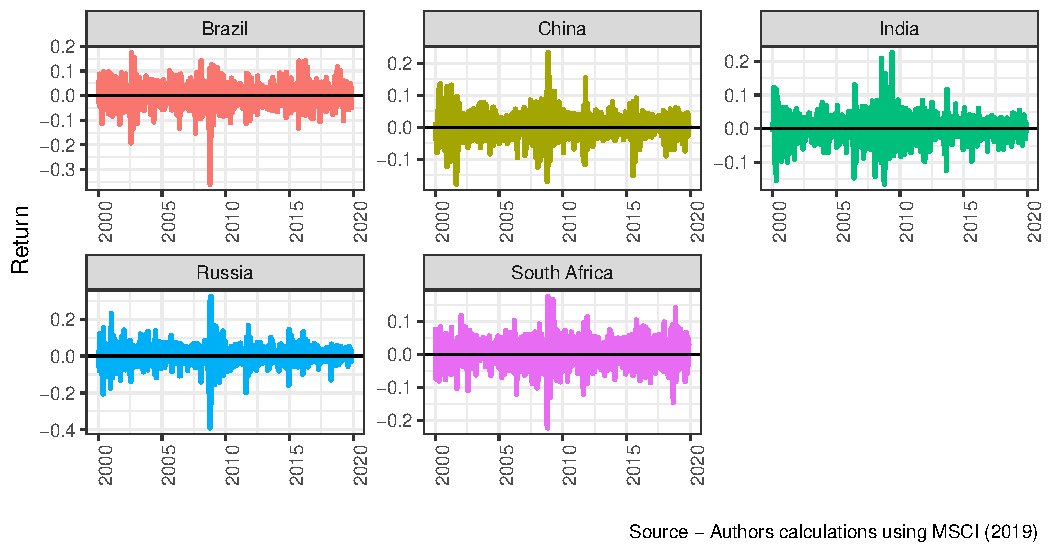
\includegraphics{Template_files/figure-latex/figreturns-1} 

}

\caption{Weekly Equity Returns - BRICS  \label{figreturns}}\label{fig:figreturns}
\end{figure}

\begin{figure}[H]

{\centering 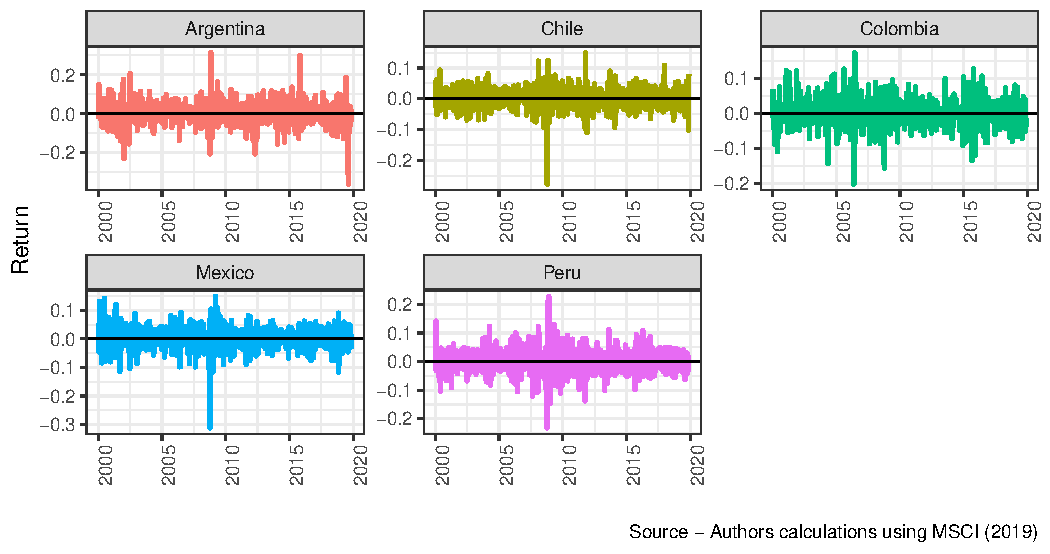
\includegraphics{Template_files/figure-latex/figreturns2-1} 

}

\caption{Weekly Equity Returns - Latin America \label{figreturns2}}\label{fig:figreturns2}
\end{figure}

\begin{figure}[H]

{\centering 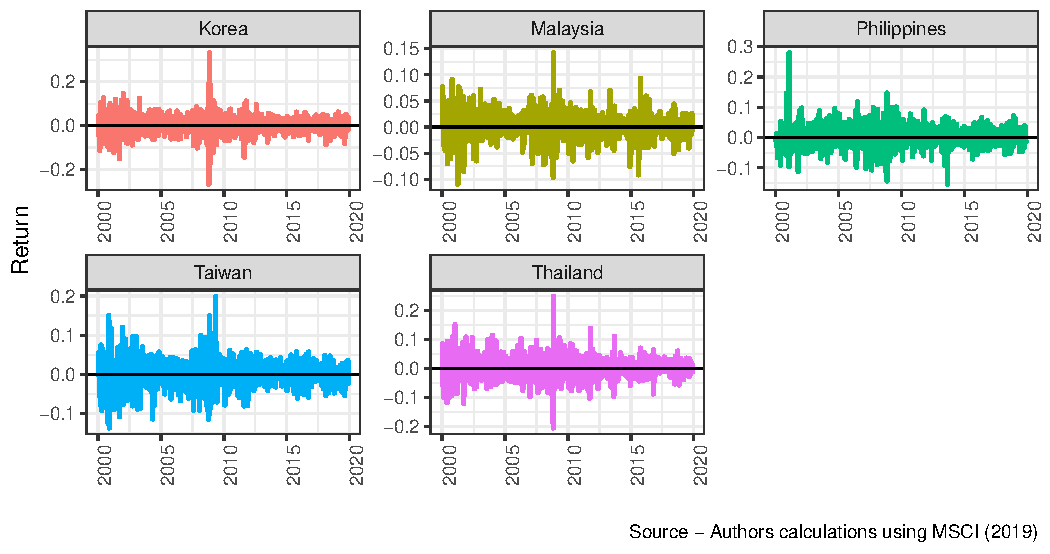
\includegraphics{Template_files/figure-latex/figreturns3-1} 

}

\caption{Weekly Equity Returns - Asia \label{figreturns3}}\label{fig:figreturns3}
\end{figure}

\begin{figure}[H]

{\centering 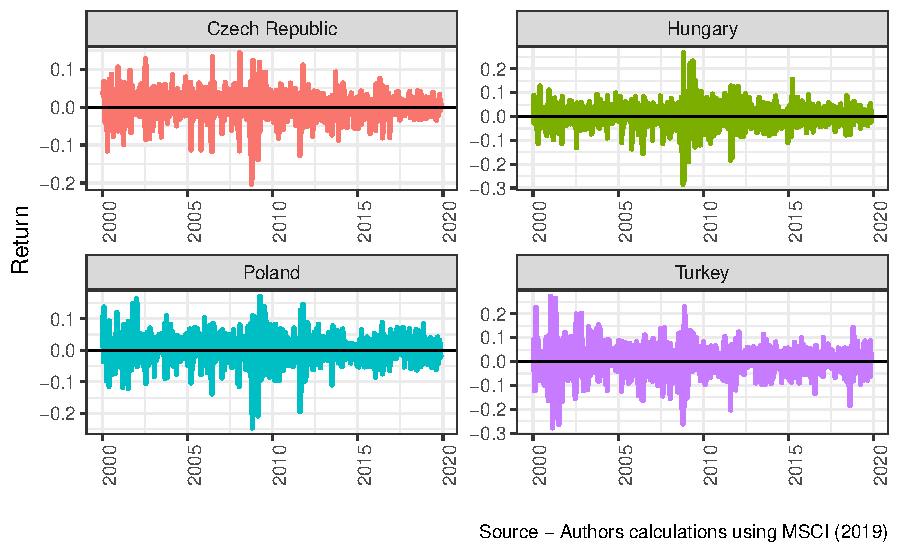
\includegraphics{Template_files/figure-latex/figreturns4-1} 

}

\caption{Weekly Equity Returns - Europe \label{figreturns4}}\label{fig:figreturns4}
\end{figure}

In assessing whether higher global uncertainty intensifies the
co-movement between these equity indices, the paper proxies this
uncertainty through the CBOE Volatility Index (VIX).\footnote{The VIX
  proxies the market's expectation of future volatility on S\&P500
  options.} The VIX has been used as a measure for global financial
market volatility in several papers such as Rey
(\protect\hyperlink{ref-rey2015dilemma}{2015}) and Friedrich and Guérin
(\protect\hyperlink{ref-friedrich2016dynamics}{2016}), which supports
its inclusion in this study. In absolute terms, a VIX above 20 typically
implies that the market is forecasting a high risk environment, with
values below 20 considered as stable. This model employs a different
approach in defining periods of high and low uncertainty, by stratifying
the VIX into quintiles and analysing the correlations between indices in
the event that these quintiles are breached. An assumption is imposed
where the VIX is required to have breached the top or bottom quintile
for a minimum of 30 trading days in order for a high/low uncertainty
period to be characterised. This will ensure that the bivariate
correlation pairs presented in table \ref{pairwise} are estimated with a
sufficient number of observations in these periods. Additionally, the
initial 10 trading days are omitted in the conditional correlation mean
calculations to allow for an adjustment period in sentiment. The VIX
over the past two decades is presented in figure \ref{figVIX}, with the
periods of high and low uncertainty shaded in pink. Due to the surge in
the VIX during the global financial crisis, all of the weekly returns
and VIX observations falling between the first day of 2008 and the final
day of 2009 are ignored in the model to avoid biased estimates in the
post crisis period.

\begin{figure}[H]

{\centering 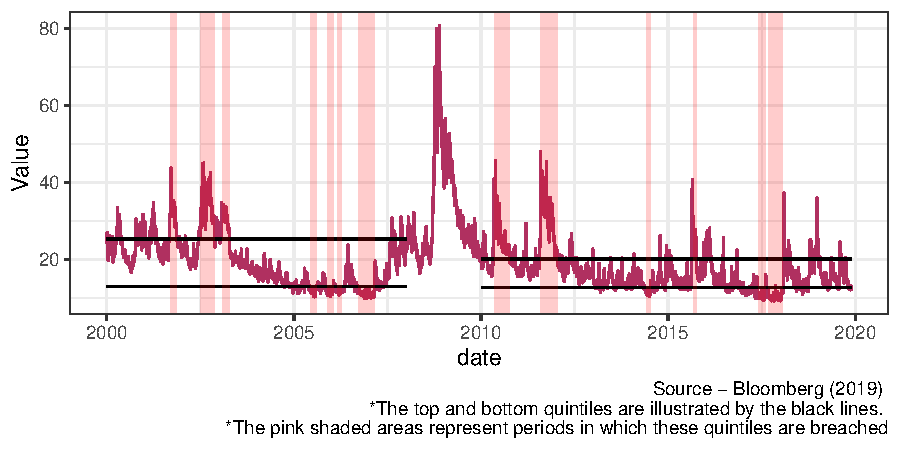
\includegraphics{Template_files/figure-latex/figVIX-1} 

}

\caption{CBOE Volatility Index (VIX) \label{figVIX}}\label{fig:figVIX}
\end{figure}

\hypertarget{methodology}{%
\section{\texorpdfstring{Methodology
\label{Methodology}}{Methodology }}\label{methodology}}

An extensive range of techniques have been applied in previous research
to model the correlations in asset returns within a portfolio. The
standard method for estimating correlations in portfolio analytics has
been the moving average specification of errors in a time series. Though
a relatively simple process to estimate, this method has fallen out of
favour in recent years due to its flawed assumption that past error term
observations are weighted equally. Bollerslev
(\protect\hyperlink{ref-bollerslev1990modelling}{1990}) pioneered the
analysis of correlations in the multivariate GARCH framework by
developing the constant conditional correlation (CCC) model, where
univariate GARCH models are computed for each asset followed by the
estimation of the correlation matrix. Even though this idea of
correlation coefficients being constant over time was deemed as
plausible in his paper, recent studies have found this property to be
unrealistic across certain asset types (see Tsui \& Yu,
\protect\hyperlink{ref-tsui1999constant}{1999}). This gave rise to the
modification of this framework by Engle
(\protect\hyperlink{ref-engle2002dynamic}{2002}), widely known as the
dynamic conditional correlation (DCC) GARCH model.\footnote{In his
  seminal paper, Engle (\protect\hyperlink{ref-engle2002dynamic}{2002})
  relaxes the constant constraint by allowing these coefficients to vary
  over time.} This seminal model forms the basis for the estimation
framework used in this paper.

The selection of this approach is based on two reasons. Firstly, the
empirical performance of DCC models are well documented, which is
underpinned in Martens and Poon
(\protect\hyperlink{ref-martens2001returns}{2001}) as well as Laurent,
Rombouts, and Violante
(\protect\hyperlink{ref-laurent2012forecasting}{2012}). Secondly, opting
for this approach will ensure parsimony. Considering that most
conditional volatility and correlation analyses are multivariate in
nature, a flexible approach is required to avoid the curse of
dimensionality faced when a large number of coefficients need to be
estimated. Instead of estimating the covariance matrix and deriving
conditional correlations from it, the DCC model estimates the
correlation matrix directly through using standardised residuals. This
is advantageous as the number of parameters which need to be estimated
are reduced when using this method.

In this study, DCC coefficients are estimated between the South African
equity index and the remaining EME equity indices in the sample, which
follows a three step process. In the first step, financial returns on
each equity index are calculated at a weekly frequency before employing
a demeaning process to derive residuals from these returns (Engle
\& Sheppard, \protect\hyperlink{ref-engle2001theoretical}{2001}). As
highlighted previously, the rationale behind opting for weekly return
computations as opposed to daily returns is predicated on avoiding the
noise in the data which could occur at such a high frequency.
Furthermore, extreme observations in each of the returns are cleaned
using a technique developed by Boudt, Peterson, and Croux
(\protect\hyperlink{ref-boudt2008estimation}{2008}), which will improve
the robustness in the risk estimates. The regression model which is
employed for these returns follows a stochastic process, specified below

\begin{equation}
r_t = a_0 + {a_1}{r_{t-1}} + \varepsilon_t
\label{eq1}
\end{equation}

where \(r_t\) represents the weekly returns on each equity index in the
model and \(\varepsilon_t\) is a k x 1 vector of the residual returns in
\(r_t\).\footnote{k denotes the number of equity indices used in the
  model.}

The second step involves the estimation of parameters in the variance
models with the use of the residuals derived in equation \ref{eq1}. The
standard multivariate GARCH framework is applied, where equity returns
are assumed to be conditionally multivariate normal with zero expected
value and a k x k time-varying covariance matrix, \(H_t\)

\begin{equation}
\varepsilon_t = D_t \upsilon_t \sim N(0, H_t)
\label{eq2}
\end{equation}

where \(D_t\) represents a k x k diagonal matrix of dynamic standard
deviations in the residual returns, and \(\upsilon_t\) represents a
column vector of standardised residual returns. Moreover, \(H_t\) takes
on the following form

\begin{equation}
H_t = D_t R_t D_t
\label{eq3}
\end{equation}

where \(R_t\) is a k x k matrix of time-varying conditional correlation
coefficients. This dynamic property serves as the main modification of
the CCC model which was discussed earlier. The variances are derived
through a first order univariate GARCH (1,1) process, as follows

\begin{equation}
h_t = b_0 + b_1\varepsilon_{t-1}^{2} + b_2\varepsilon_{t-1}^{2}
\label{eq4}
\end{equation}

The log-likelihood function to determine the parameters in equations
\ref{eq4} and \ref{eq7} is given by

\begin{align} \label{eq5}
l &= -0.5 \sum_{t=1}^{T}[n log(2\pi) + log(\mid H_t \mid) + \varepsilon_t^{'} H_t \varepsilon_t] \hfill  \\ \notag
                     &= -0.5 \sum_{t=1}^{T}[n log(2\pi) + log(\mid D_t R_t D_t \mid) + \upsilon_t^{'}D_t^{-1}R_t^{-1}D_t^{-1}\upsilon_t] \notag
                           \end{align}

Thereafter, the following can be considered

\begin{align} \label{eq6}
 \varepsilon_t^{'} D_t^{-2} \varepsilon_t &=  \varepsilon_t^{'} D_t^{-1} D_t^{-1} \varepsilon_t = [D_t^{-1} \varepsilon_t]^{'}D_t^{-1}\varepsilon_t = \upsilon_t^{'}\upsilon_t, \hfill  \\ \notag
                     l &= -0.5 \sum_{t=1}^{T} [nlog(2\pi) + 2log( \mid D_t \mid) + \varepsilon_t^{'} D_t^{-2} \varepsilon_t] -0.5 \sum_{t=1}^{T} [log(\mid R_t \mid) + \varepsilon_t^{'}R_t^{-1} \varepsilon_t - \upsilon_t^{'}\upsilon_t] \hfill \\ \notag
                     &= l_1 + l_2
                           \end{align}

where:

\begin{equation}
l_1 = -0.5 \sum_{t=1}^{T}[nlog(2\pi) +  2 log(\mid D_t \mid ) + \varepsilon_t^{'} D_t^{-2} \varepsilon_t]
\label{eq7}
\end{equation}

and

\begin{equation}
l_2= -0.5 \sum_{t=1}^{T} [log(\mid R_t \mid ) + \varepsilon_t^{'}R_t^{-1}\varepsilon_t - \upsilon_t^{'}\upsilon_t]
\label{eq8}
\end{equation}

Equations \ref{eq7} and \ref{eq8} show that the log-likelihood function
can be decomposed into functions of variances and correlations. The
parameters of variances in \(l_t\) are determined without simultaneous
determinations of the correlation parameters by maximising \(l_t\).

The third and final step in the model involves the estimation of
correlation coefficients. The correlation coefficients between equity
index returns \(i\) and \(j\) at period \(t\) can be expressed as
follows

\begin{equation}
\rho_{ijt} = \frac{E_{t-1}[\varepsilon_{it}\varepsilon_{jt}]}{\sqrt{E_{t-1}[\varepsilon_{it}^2]} \sqrt{E_{t-1}[\varepsilon_{jt}^2]}} = \frac{E_{t-1}[\sqrt{h_{it}}\upsilon_{1t}\sqrt{h_{jt}} \upsilon_{jt}]}{\sqrt{E_{t-1}[h_{it}v_{it}^2]}\sqrt{E_{t-1}[h_{jt}v_{it}^2]}} = \frac{E_{t-1}[v_{it}v_{it}]}{\sqrt{E_{t-1}[v_{it}^2]}\sqrt{E_{t-1}[v_{jt}^2]}} = E_{t-1}[v_{it}v_{jt}]
\label{eq9}
\end{equation}

where \begin{equation}
E_{t-1}[\upsilon_{it}^2] = E_{t-1}[h_{it}^{-1}\varepsilon_{it}^2] = h_{it}^{-1}E_{t-1}[\varepsilon_{it}^2] = 1
\label{eq15}
\end{equation}

The correlation coefficients in \(\rho_{ijt}\) form the correlation
matrix \(R_t\), where its diagonal elements are equal to 1.

If the unconditional variance estimate used in the model (denoted by
\(Q_t\)) can be expressed by the following

\begin{equation}
Q_{t} = E_{t-1}[\upsilon_t\upsilon_t{'}]
\label{eq10}
\end{equation}

then \(R_t\) can be rewritten as

\begin{equation}
R_{t} = [diag(Q_t)]^{-\frac{1}{2}} Q_t[diag(Q_t)]^{-\frac{1}{2}} 
\label{eq11}
\end{equation}

Thereafter, the correlation coefficient \(\rho_t\) should be
parameterised. For this to be achieved, the model assumes that \(Q_t\)
follows an autoregressive process. This would entail that

\begin{equation}
Q_{t} = \overline{Q} (1 - \alpha - \beta) + \alpha \upsilon_{t-1} \upsilon_{t-1}^{'} + \beta Q_{t-1}
\label{eq12}
\end{equation}

where \(\alpha\) and \(\beta\) are scalar parameters which capture the
effects of past shocks and DCCs on current DCCs. In the case of the
DCC(1,1), \(\alpha\) and \(\beta\) are positive and \(\alpha\) +
\(\beta\) \textless{} 1, which ensures that \(Q_t\) is positive and
mean-reverting. This property implies that in the event of a shock, the
correlation between the underlying assets will return to its long run
unconditional level. \(\overline{Q}\) is an unconditional correlation
coefficient matrix. The unconditional correlations are determined in the
second step and used as predetermined values in this step (Engle \&
Sheppard, \protect\hyperlink{ref-engle2001theoretical}{2001}). The
parameters for the dynamic correlations are derived by maximising the
log likelihood function \(l_2\). Considering that
\(\upsilon_t^{'} \upsilon_t\) does not involve the determination of
parameters, the log likelihood function can be reduced to

\begin{equation}
l_2 = -0.5 \bullet_{t=1}^{T} [log(R_t) + \varepsilon_t^{'} R_t^{-1} \varepsilon_t]
\label{eq13}
\end{equation}

Finally, the correlation model in equation \ref{eq12} can be used to
estimate the co-movement in equity indices by pairing the South African
equity index with the remaining indices in the sample. As highlighted
previously, these co-movements are studied generally before analysing
them under high and low uncertainty episodes to form conclusions of
contagion effects arising from implied volatility on the S\&P500. The
findings from the correlation pairs are presented throughout section
\ref{Results}.

\hypertarget{results}{%
\section{\texorpdfstring{Results
\label{Results}}{Results }}\label{results}}

The summary statistics for the weekly equity returns in all of the EMEs
considered in this paper are presented in table \ref{summarystats}. The
mean returns prior to the onset of the global financial crisis range
from 0.68\% in Colombia and the Czech Republic, with the Philippines and
Taiwan reporting the lowest mean returns of 0.19\% and 0.06\%
respectively. Notably, these average weekly returns were higher during
this period when contrasted with the post crisis period across all of
the sample economies. This should be expected, given the sharp
deceleration in portfolio flows to EMEs immediately after the financial
crisis (largely fuelled by a rise in global risk aversion), as well the
more recent equity outflow episodes which EMEs have experienced since
the Taper Tantrum in 2013 (see Milesi-Ferretti \& Tille,
\protect\hyperlink{ref-milesi2011great}{2011}; Sahay \emph{et al.},
\protect\hyperlink{ref-sahay2014emerging}{2014}). The standard
deviation values in this pre-crisis period indicate that Turkish and
Russian equity markets have displayed the greatest degree of risk.
Surprisingly, lower standard deviation scores were reported in all of
the economies after the financial crisis (with the exception of
Argentina and Hungary), contrary to the consensus which suggests that
financial markets have been more volatile throughout the post-Lehman era
(see Grima \& Caruana, \protect\hyperlink{ref-grima2017effect}{2017}).
This finding on Argentina in the post crisis period is best explained as
a result of interest rate hikes which their central bank has had to
employ in attempt to counteract the high inflation episodes they've
faced in recent years.\footnote{Cachanosky and Ferrelli-Mazza
  (\protect\hyperlink{ref-cachanosky2019did}{2019}) highlighted these
  high policy interest rates coupled with an increase in sovereign
  default risk and devaluations in the peso as core reasons behind the
  recent surge in speculative activity across Argentinean financial
  markets.}

The estimation of conditional volatilities provides further insight into
the dynamics within equity returns over the past two decades. From
figures \ref{bricsvol} - \ref{vol.europe}, it is evident that the BRICS
and Latin American economies have been characterised by substantial
levels in equity market volatility (notably in Argentina, Brazil as well
as a recent surge in South African conditional volatility). This finding
should bear concerns for investors with investment exposure in these
economies. The effects caused by the Taper Tantrum are most evident in
the BRICS and Asian economies, seen by an uptick in conditional
volatility between 2013 and 2015 when analysing these plots closely. In
the Asian region, the lowest conditional volatility is seen in the
Malaysian case. Interestingly, the conditional volatilities throughout
the Asian region were lower in the post crisis period when contrasted to
prior to 2008. Similar sentiments related to lower Asian equity market
conditional volatility in the post crisis era are found in Roni, Abbas,
and Wang (\protect\hyperlink{ref-roni2018return}{2018}).

\begin{figure}[H]

{\centering 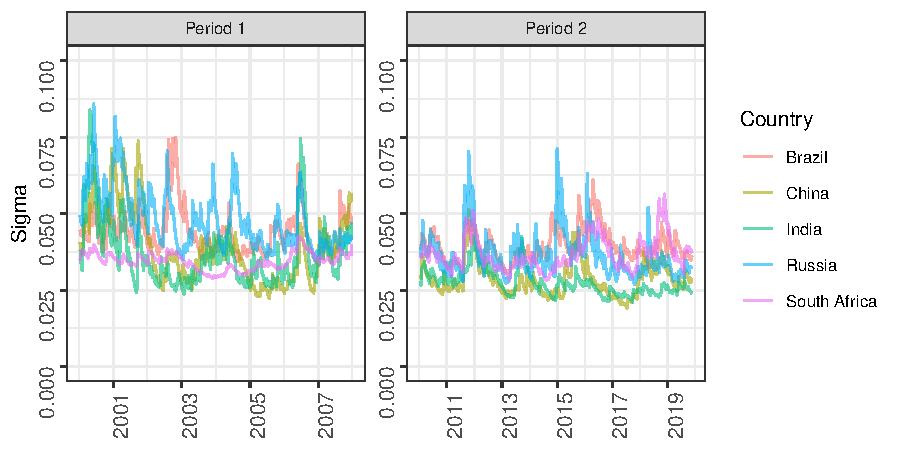
\includegraphics{Template_files/figure-latex/volplotbrics-1} 

}

\caption{BRICS conditional volatility \label{bricsvol}}\label{fig:volplotbrics}
\end{figure}

\begin{figure}[H]

{\centering 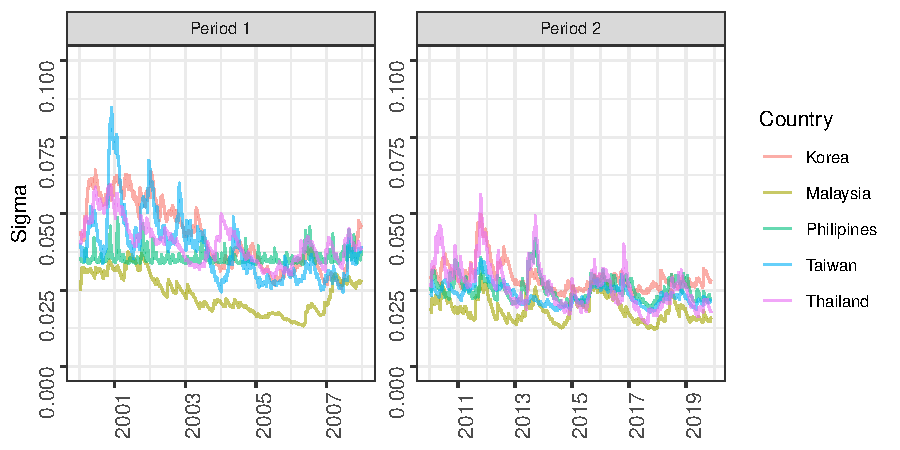
\includegraphics{Template_files/figure-latex/vol2-1} 

}

\caption{Asia Conditional Volatility \label{vol.asia}}\label{fig:vol2}
\end{figure}

\begin{figure}[H]

{\centering 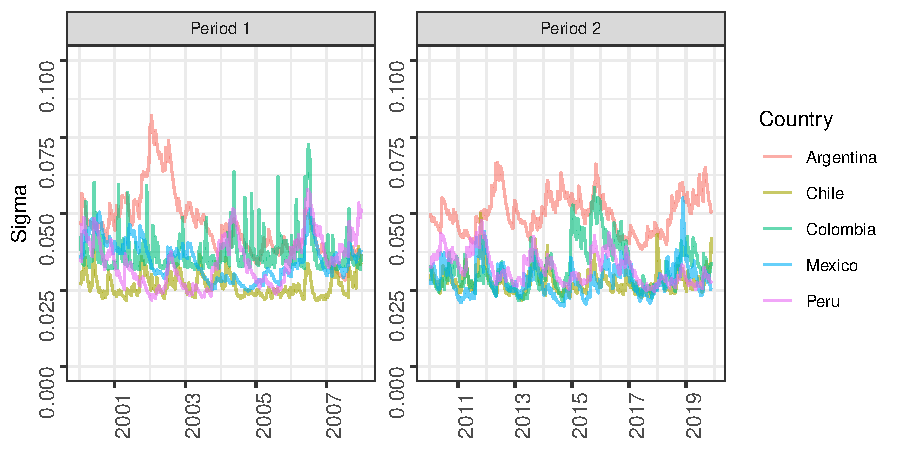
\includegraphics{Template_files/figure-latex/vol3-1} 

}

\caption{Latin America Conditional Volatility \label{vol.south.america}}\label{fig:vol3}
\end{figure}

\begin{figure}[H]

{\centering 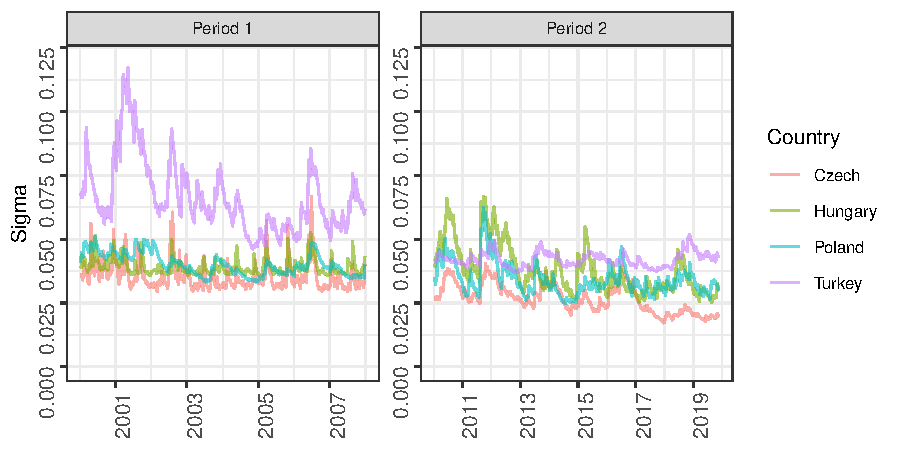
\includegraphics{Template_files/figure-latex/vol4-1} 

}

\caption{Europe Conditional Volatility \label{vol.europe}}\label{fig:vol4}
\end{figure}

In analysing the bivariate correlations between the South African equity
index and the remaining EMEs represented in figures \ref{dcc1} -
\ref{dcc4}, almost all cases experienced a considerable rise in
correlation between the pre and post crisis period. Kryzanowski, Zhang,
and Zhong (\protect\hyperlink{ref-kryzanowski2017cross}{2017}) support
this finding with their conclusion on the rise in EME equity
correlations occuring in the aftermath of the first two phases of
QE.\footnote{This phenomenon entails that the large scale asset
  purchases carried out by the major central banks such as the Fed and
  ECB have driven asset prices in EMEs closer to each other.} The
correlations between the South African equity market and majority of the
EMEs studied in this paper are estimated to hover around the 0.5 mark
since the crisis. In interpreting this, it can be expected that a 1\%
increase in the South African equity index will coincide with an atleast
0.5\% rise on a corresponding EME equity index. The highest correlations
are seen in the relationship between the South African index with Chile,
Mexico, China, Korea and Poland. Also, it appears that the Argentinean
case in conjunction with three of the four European EMEs exhibit the
lowest degree of correlation with South Africa across the sample.
Naturally, these co-movements pose the challenge for investors to
successfully hedge their portfolios through exposure in different EMEs.
These high correlations should also be of concern to policymakers in
these economies when weighing up considerations of liberalising their
capital markets, as the inter-connectedness in these indices serves as
an indication that volatility in another EME can result in spillover
effects in their local financial markets.

\begin{figure}[H]

{\centering 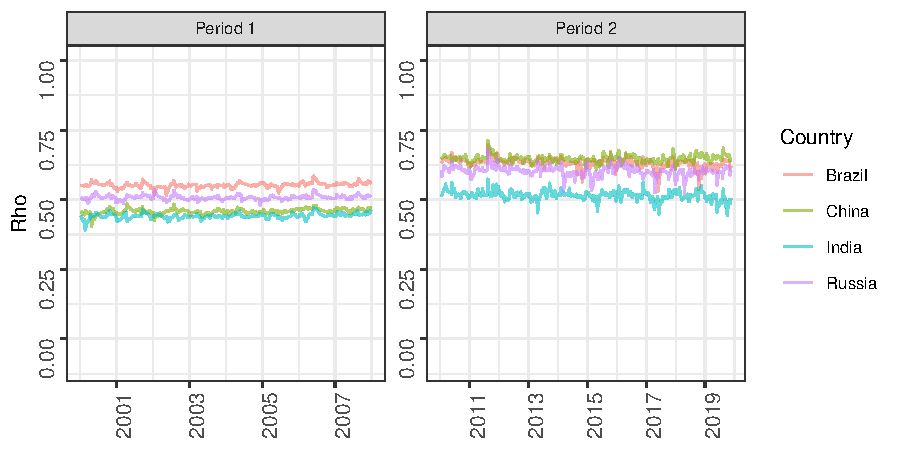
\includegraphics{Template_files/figure-latex/dcc1-1} 

}

\caption{South Africa-BRICS DCC \label{dcc1}}\label{fig:dcc1}
\end{figure}
\begin{figure}[H]

{\centering 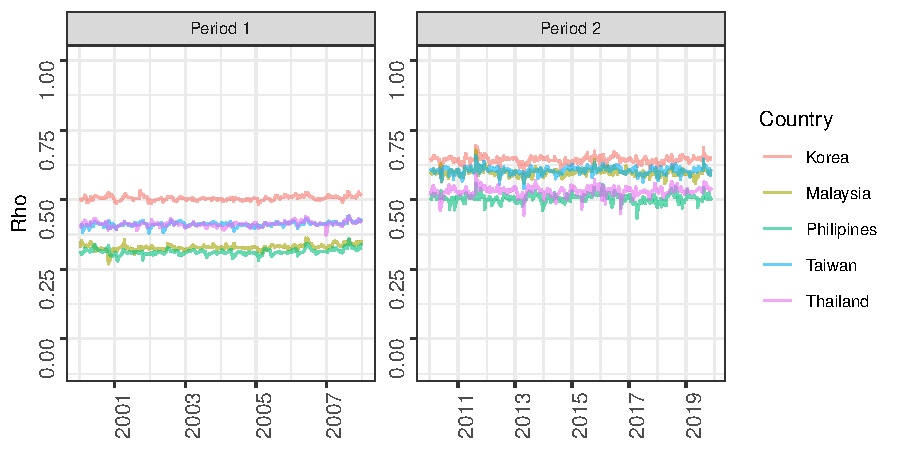
\includegraphics{Template_files/figure-latex/dcc2-1} 

}

\caption{South Africa-Asia DCC \label{dcc2}}\label{fig:dcc2}
\end{figure}
\begin{figure}[H]

{\centering 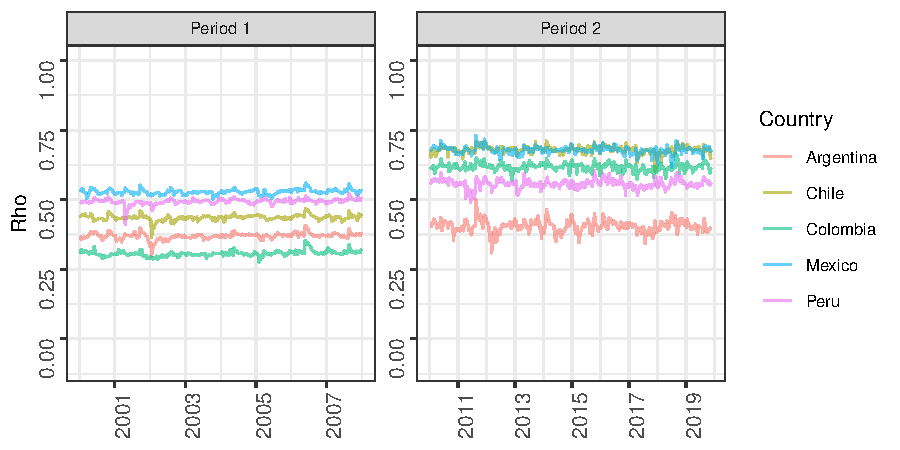
\includegraphics{Template_files/figure-latex/dcc3-1} 

}

\caption{South Africa-Latin America DCC \label{dcc3}}\label{fig:dcc3}
\end{figure}
\begin{figure}[H]

{\centering 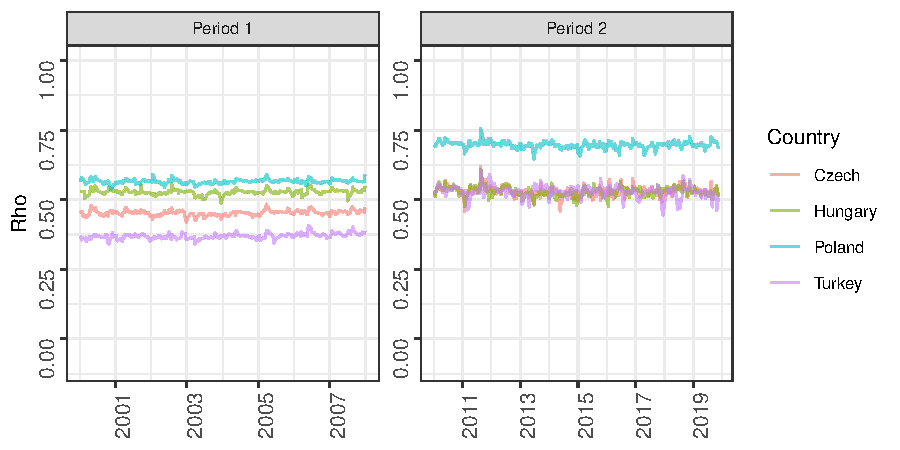
\includegraphics{Template_files/figure-latex/dcc4-1} 

}

\caption{South Africa-Europe DCC\label{dcc4}}\label{fig:dcc4}
\end{figure}

Interestingly, the findings suggest that correlations do not differ
considerably during periods of low and high global uncertainty, contrary
to the findings in Cappiello, Engle, and Sheppard
(\protect\hyperlink{ref-cappiello2006asymmetric}{2006}) as well as
Sarwar and Khan (\protect\hyperlink{ref-sarwarimpact}{2017}). Figures
\ref{dcc6} - \ref{dcc9} illustrate the correlations discussed with the
shaded areas representing the periods of low and high volatility
specified in the model. It appears that the bivariate correlations
remain relatively constant when intersecting with the high VIX episodes
in both the pre and post crisis period, which serves as an indication
that higher implied US stock market volatility does not necessarily
intensify the inter-connectedness in these equity returns. Table
\ref{pairwise} reports the average correlation pairs during the high and
low VIX periods, where they are estimated to be relatively similar in
both cases. Therefore, international investors can take some consolation
from this finding as the spillover effects from the US stock market
volatility do not appear to have had a substantial impact on equity
correlations across the sample.

Overall, the findings uncovered throughout this section are bound to
have considerable implications for both international investor as well
as policymaking decisions. From a international investor perspective,
the rationale behind investing in EMEs is predicated on being able to
maximise asset returns while contemporaneously minimising the risk
associated with these assets. Markowitz
(\protect\hyperlink{ref-markowitz1952portfolio}{1952}) pioneered the
idea of portfolio diversification in emphasizing that the holdings
within a portfolio should not be strongly correlated. In this sense, the
findings uncovered in the bivariate pairs suggest that investors have
less scope to diversify their portfolios purely through investing in
different EMEs. This notion has been emphasised in the post-Lehman era
when contrasted with the correlations prior to the crisis' onset.
Furthermore, the high correlations between these assets should be of
particular importance to policymakers who are aiming to navigate their
economies around the risk of contagion and capital flow volatility
through using macro-prudential tools.

\hypertarget{conclusion}{%
\section{\texorpdfstring{Conclusion
\label{Conclusion}}{Conclusion }}\label{conclusion}}

This paper offers a perspective on the conditional volatility and the
inter-connectedness exhibited in the returns on equity indices across
EMEs. Through employing a multivariate DCC-GARCH approach, the magnitude
in correlations between returns on the South African equity index and 18
of its EME counterparts are analysed extensively. Furthermore, this
research focuses on the possible contagion effects which arise in these
economies due to higher US equity market volatility, where the dynamics
in these co-movements during high VIX periods are assessed. The main
findings uncovered in the paper suggest that the bivariate correlations
between South Africa and most of the EMEs in question have risen
substantially since the global financial crisis, as well as limited
evidence to suggest that equity co-movements have been heightened during
periods of high implied volatility. From a conditional volatility
perspective, the Asian region and isolated cases such as the Czech
Republic and Turkey have exhibited a decline during the post-Lehman era.

The higher correlations between these equity pairs suggest that
policymakers should respond to negative shocks with an improvement in
macroeconomic fundamentals in their respective economies. Therefore, it
is crucial for policymakers to build an understanding on the underlying
mechanisms which drive these co-movements for appropriate policy
decisions to be carried out. If they fail to factor these
characteristics into their decision process, it is possible that they
will end up doing worse rather than better. One can argue that the Fed
(through improved forward guidance) and the IMF (by intervening with
balance of payments support) should have a greater responsibility in
insulating EMEs which are most vulnerable to contagion. In explaining
the implications these findings have on international portfolio
management, investors should realise that their pursuit for arbitrage
opportunities and portfolio diversification requires a more holistic
approach than merely spreading a portfolio across different EMEs. The
sizing of an allocation and employing long-horizon investment strategies
could be crucial in counteracting these risks highlighted above (see
Viceira \& Wang, \protect\hyperlink{ref-viceira2018global}{2018}; Scott \emph{et al.},
\protect\hyperlink{ref-scott2019global}{2019})


Conclusively, interesting extensions for this research in the future
could be achieved by testing for contagion across multiple asset
classes, as well as investigating the role which institutional investors
(such as hedge funds and mutual funds) have had in fuelling these
increases in risk. Furthermore, the use of block-structure parameter
matrices can improve the robustness of the estimates while preserving
the simplicity of the model, as applied in Billio, Caporin, and Gobbo
(\protect\hyperlink{ref-billio2003block}{2003}). This can be achieved
because the dynamic nature of the correlations are allowed to be non
identical across the assets in the estimation process, hence overcoming
one of the main shortcomings of the DCC-GARCH approach.

\newpage

\hypertarget{appendix}{%
\section{\texorpdfstring{Appendix
\label{Appendix}}{Appendix }}\label{appendix}}

\begin{longtable}{rllll}
\caption{List of equity indices \label{tabsample}} \\ 
  \hline
 & Country & Name & Ticker & Group \\ 
  \hline
1 & Brazil & BOVEPSA & MXBR Index & BRICS \\ 
  2 & Russia & MOEX & MXRU Index & BRICS \\ 
  3 & India & SENSEX & MXIN Index & BRICS \\ 
  4 & China & SSE Composite Index & MXCN Index & BRICS \\ 
  5 & South Africa & JSE Top 40 & MXZA Index & BRICS \\ 
  6 & Mexico & IPC & MXMX Index & Latin America \\ 
  7 & Argentina & MERVAL Index & MXAR Index & Latin America \\ 
  8 & Chile & IPSA Index & MXCL Index & Latin America \\ 
  9 & Colombia & COLCAP Index & MXCO Index & Latin America \\ 
  10 & Peru & IGBVL Index & MXPE Index & Latin America \\ 
  11 & Taiwan & TWSE Index & TAMSCI Index & Asia \\ 
  12 & Thailand & SET 50 & MXTH Index & Asia \\ 
  13 & Philipines & PSEi Index & MXPH Index & Asia \\ 
  14 & Malaysia & FTSE KLCI & MXMY Index & Asia \\ 
  15 & Korea & KOPSI Index & MXKR Index & Asia \\ 
  16 & Czech & PSE PX & MXCZ Index & Europe \\ 
  17 & Hungary & BUX Index & MXHU Index & Europe \\ 
  18 & Poland & SIX & MXPL Index & Europe \\ 
  19 & Turkey & XU100 & MXTR Index & Europe \\ 
   \hline
\hline
\end{longtable}

\begin{longtable}{rlrrrr}
\caption{Equity Returns Summary Statistics \label{summarystats}} \\ 
  \hline
 & Ticker & Mean Period 1 & SD Period 1 & Mean Period 2 & SD Period 2 \\ 
  \hline
1 & MXAR Index & 0.0030 & 0.0490 & 0.0010 & 0.0537 \\ 
  2 & MXBR Index & 0.0053 & 0.0454 & 0.0004 & 0.0401 \\ 
  3 & MXCL Index & 0.0032 & 0.0268 & -0.0001 & 0.0290 \\ 
  4 & MXCN Index & 0.0037 & 0.0410 & 0.0013 & 0.0304 \\ 
  5 & MXCO Index & 0.0068 & 0.0404 & 0.0006 & 0.0333 \\ 
  6 & MXCZ Index & 0.0068 & 0.0360 & 0.0002 & 0.0277 \\ 
  7 & MXHU Index & 0.0041 & 0.0398 & 0.0013 & 0.0401 \\ 
  8 & MXIN Index & 0.0045 & 0.0388 & 0.0010 & 0.0285 \\ 
  9 & MXKR Index & 0.0038 & 0.0441 & 0.0013 & 0.0300 \\ 
  10 & MXMX Index & 0.0040 & 0.0358 & 0.0005 & 0.0287 \\ 
  11 & MXMY Index & 0.0027 & 0.0254 & 0.0007 & 0.0198 \\ 
  12 & MXPE Index & 0.0063 & 0.0358 & 0.0014 & 0.0329 \\ 
  13 & MXPH Index & 0.0019 & 0.0380 & 0.0021 & 0.0266 \\ 
  14 & MXPL Index & 0.0039 & 0.0413 & 0.0006 & 0.0361 \\ 
  15 & MXRU Index & 0.0063 & 0.0506 & 0.0015 & 0.0390 \\ 
  16 & MXTH Index & 0.0031 & 0.0413 & 0.0024 & 0.0279 \\ 
  17 & MXTR Index & 0.0038 & 0.0698 & 0.0000 & 0.0430 \\ 
  18 & MXZA Index & 0.0036 & 0.0349 & 0.0012 & 0.0374 \\ 
  19 & TAMSCI Index & 0.0006 & 0.0405 & 0.0018 & 0.0239 \\ 
   \hline
\hline
\end{longtable}

\begin{longtable}{rllllrrr}
\caption{Average pairwise correlations \label{pairwise}} \\ 
  \hline
 & Pairs & Period & Group & Country & SampleAverage & HighVIX & LowVIX \\ 
  \hline
1 & MXZA\_MXKR & Period 1 & Asia & Korea & 0.51 & 0.51 & 0.51 \\ 
  2 & MXZA\_MXKR & Period 2 & Asia & Korea & 0.64 & 0.65 & 0.64 \\ 
  3 & MXZA\_MXMY & Period 1 & Asia & Malaysia & 0.33 & 0.33 & 0.33 \\ 
  4 & MXZA\_MXMY & Period 2 & Asia & Malaysia & 0.60 & 0.60 & 0.59 \\ 
  5 & MXZA\_MXPH & Period 1 & Asia & Philipines & 0.31 & 0.31 & 0.31 \\ 
  6 & MXZA\_MXPH & Period 2 & Asia & Philipines & 0.51 & 0.51 & 0.50 \\ 
  7 & MXZA\_TAMSCI & Period 1 & Asia & Taiwan & 0.41 & 0.42 & 0.41 \\ 
  8 & MXZA\_TAMSCI & Period 2 & Asia & Taiwan & 0.60 & 0.61 & 0.60 \\ 
  9 & MXZA\_MXTH & Period 1 & Asia & Thailand & 0.41 & 0.42 & 0.41 \\ 
  10 & MXZA\_MXTH & Period 2 & Asia & Thailand & 0.53 & 0.53 & 0.53 \\ 
  11 & MXZA\_MXBR & Period 1 & BRICS & Brazil & 0.55 & 0.55 & 0.55 \\ 
  12 & MXZA\_MXBR & Period 2 & BRICS & Brazil & 0.63 & 0.65 & 0.62 \\ 
  13 & MXZA\_MXCN & Period 1 & BRICS & China & 0.46 & 0.46 & 0.46 \\ 
  14 & MXZA\_MXCN & Period 2 & BRICS & China & 0.65 & 0.65 & 0.64 \\ 
  15 & MXZA\_MXIN & Period 1 & BRICS & India & 0.44 & 0.44 & 0.44 \\ 
  16 & MXZA\_MXIN & Period 2 & BRICS & India & 0.52 & 0.53 & 0.51 \\ 
  17 & MXZA\_MXRU & Period 1 & BRICS & Russia & 0.51 & 0.51 & 0.51 \\ 
  18 & MXZA\_MXRU & Period 2 & BRICS & Russia & 0.60 & 0.62 & 0.60 \\ 
  19 & MXZA\_MXCZ & Period 1 & Europe & Czech & 0.45 & 0.45 & 0.45 \\ 
  20 & MXZA\_MXCZ & Period 2 & Europe & Czech & 0.53 & 0.55 & 0.52 \\ 
  21 & MXZA\_MXHU & Period 1 & Europe & Hungary & 0.53 & 0.53 & 0.53 \\ 
  22 & MXZA\_MXHU & Period 2 & Europe & Hungary & 0.53 & 0.54 & 0.53 \\ 
  23 & MXZA\_MXPL & Period 1 & Europe & Poland & 0.57 & 0.57 & 0.57 \\ 
  24 & MXZA\_MXPL & Period 2 & Europe & Poland & 0.70 & 0.71 & 0.69 \\ 
  25 & MXZA\_MXTR & Period 1 & Europe & Turkey & 0.37 & 0.37 & 0.37 \\ 
  26 & MXZA\_MXTR & Period 2 & Europe & Turkey & 0.53 & 0.55 & 0.52 \\ 
  27 & MXZA\_MXAR & Period 1 & Latin America & Argentina & 0.37 & 0.37 & 0.37 \\ 
  28 & MXZA\_MXAR & Period 2 & Latin America & Argentina & 0.40 & 0.42 & 0.39 \\ 
  29 & MXZA\_MXCL & Period 1 & Latin America & Chile & 0.44 & 0.43 & 0.44 \\ 
  30 & MXZA\_MXCL & Period 2 & Latin America & Chile & 0.68 & 0.69 & 0.67 \\ 
  31 & MXZA\_MXCO & Period 1 & Latin America & Colombia & 0.31 & 0.30 & 0.31 \\ 
  32 & MXZA\_MXCO & Period 2 & Latin America & Colombia & 0.62 & 0.62 & 0.61 \\ 
  33 & MXZA\_MXMX & Period 1 & Latin America & Mexico & 0.53 & 0.53 & 0.53 \\ 
  34 & MXZA\_MXMX & Period 2 & Latin America & Mexico & 0.68 & 0.69 & 0.67 \\ 
  35 & MXZA\_MXPE & Period 1 & Latin America & Peru & 0.49 & 0.49 & 0.49 \\ 
  36 & MXZA\_MXPE & Period 2 & Latin America & Peru & 0.56 & 0.57 & 0.55 \\ 
   \hline
\hline
\end{longtable}

\hypertarget{dynamic-conditional-correlations-with-uncertainty}{%
\subsection{Dynamic Conditional Correlations with
uncertainty}\label{dynamic-conditional-correlations-with-uncertainty}}

\begin{figure}[H]

{\centering 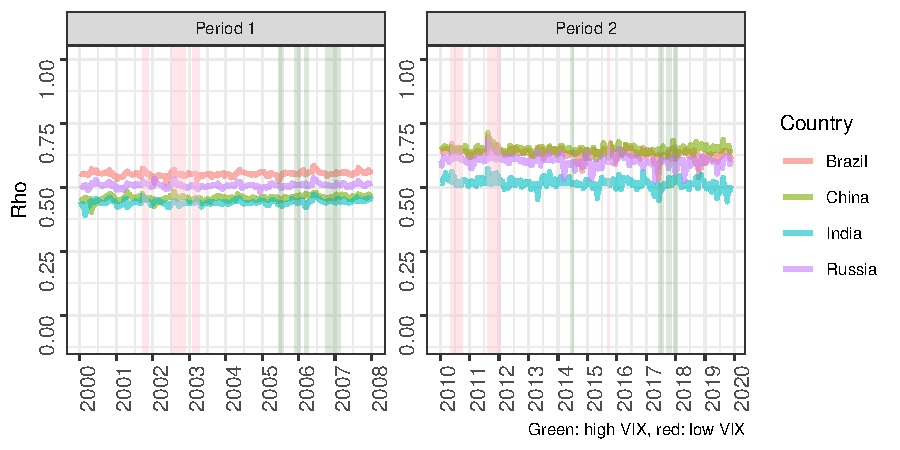
\includegraphics{Template_files/figure-latex/dcc6-1} 

}

\caption{South Africa-BRICS DCC\label{dcc6}}\label{fig:dcc6}
\end{figure}
\begin{figure}[H]

{\centering 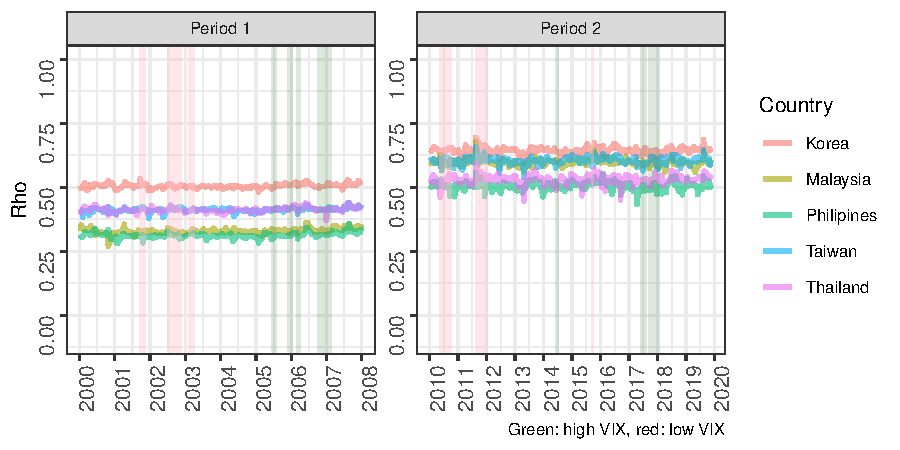
\includegraphics{Template_files/figure-latex/dcc7-1} 

}

\caption{South Africa-Asia DCC \label{dcc7}}\label{fig:dcc7}
\end{figure}
\begin{figure}[H]

{\centering 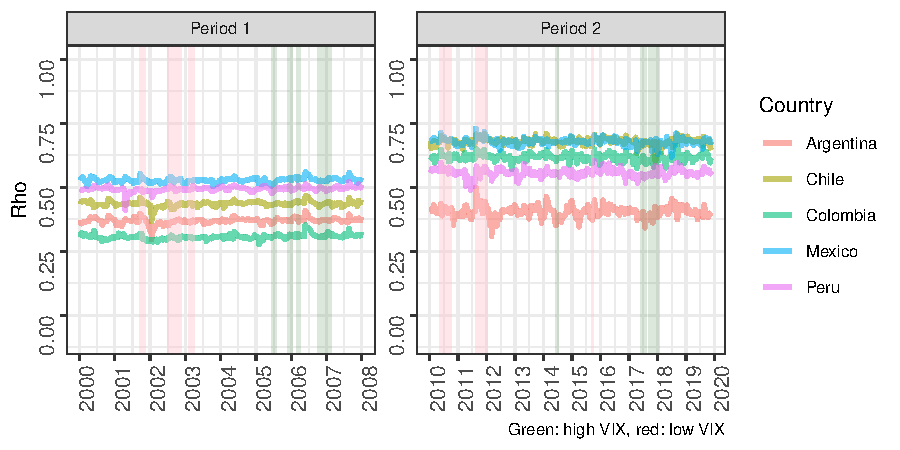
\includegraphics{Template_files/figure-latex/dcc8-1} 

}

\caption{South Africa-Latin America DCC \label{dcc8}}\label{fig:dcc8}
\end{figure}
\begin{figure}[H]

{\centering 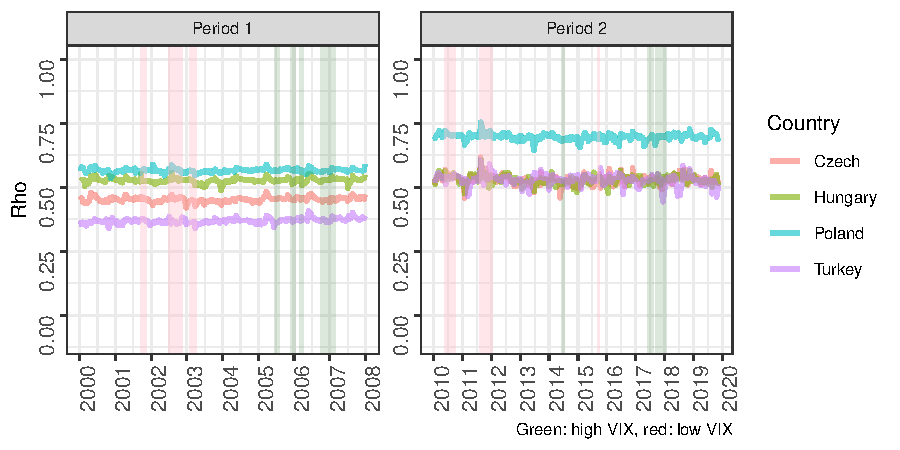
\includegraphics{Template_files/figure-latex/dcc9-1} 

}

\caption{South Africa-Europe DCC\label{dcc9}}\label{fig:dcc9}
\end{figure}

\newpage

\hypertarget{references}{%
\section*{\texorpdfstring{References
\label{References}}{References }}\label{references}}
\addcontentsline{toc}{section}{References \label{References}}

\hypertarget{refs}{}
\leavevmode\hypertarget{ref-aloui2011global}{}%
Aloui, R., Aissa, M \& Nguyen, D. 2011.
Global Financial Crisis, Extreme Interdependences, and Contagion
Effects: The Role of Economic Structure? \emph{Journal of Banking \&
Finance,} 35(1): 130--141.

\leavevmode\hypertarget{ref-bekaert2003market}{}%
Bekaert, G, \& Harvey, C. 2003. Market Integration and
Contagion. National Bureau of Economic Research.

\leavevmode\hypertarget{ref-billio2003block}{}%
Billio, M., Caporin, M \& Gobbo, M. 2003. Block
Dynamic Conditional Correlation Multivariate GARCH Models. Universita di Venezia.

\leavevmode\hypertarget{ref-bollerslev1990modelling}{}%
Bollerslev, T. 1990. Modelling the Coherence in Short-Run Nominal
Exchange Rates: A Multivariate Generalized ARCH Model. \emph{The
Review of Economics and Statistics,} 498--505.

\leavevmode\hypertarget{ref-bonga2017assessing}{}%
Bonga-Bonga, L. 2017. Assessing the Readiness of the BRICS
Grouping for Mutually Beneficial Financial Integration. \emph{Review
of Development Economics,} 21(4): 204--219.

\leavevmode\hypertarget{ref-boudt2008estimation}{}%
Boudt, K., Peterson, B., \& Croux, C. 2008. Estimation
and Decomposition of Downside Risk for Portfolios with Non-Normal
Returns. \emph{Journal of Risk,} 11(2): 79--103.

\leavevmode\hypertarget{ref-cachanosky2019did}{}%
Cachanosky, N \& Ferrelli-Mazza, F. 2019. Why Did
Inflation Targeting Fail in Argentina? American Institute for Economic Research

\leavevmode\hypertarget{ref-cappiello2006asymmetric}{}%
Cappiello, L., Engle, R \& Sheppard, K. 2006.
Asymmetric Dynamics in the Correlations of Global Equity and Bond
Returns. \emph{Journal of Financial Econometrics,} 4(4): 537--572.

\leavevmode\hypertarget{ref-carrieri2007characterizing}{}%
Carrieri, F., Errunza, V \& Hogan, K. 2007.
Characterizing World Market Integration Through Time. \emph{Journal
of Financial and Quantitative Analysis,} 42(4): 915--940.

\leavevmode\hypertarget{ref-diebold2012better}{}%
Diebold, F \& Yilmaz, K. 2012. Better to Give Than to
Receive: Predictive Directional Measurement of Volatility Spillovers.
\emph{International Journal of Forecasting,} 28(1): 57--66.

\leavevmode\hypertarget{ref-engle2002dynamic}{}%
Engle, R. 2002. Dynamic Conditional Correlation: A Simple Class
of Multivariate Generalized Autoregressive Conditional
Heteroskedasticity Models. \emph{Journal of Business \& Economic
Statistics,} 20(3): 339--350.

\leavevmode\hypertarget{ref-engle2001theoretical}{}%
Engle, R \& Sheppard, K. 2001. Theoretical and Empirical
Properties of Dynamic Conditional Correlation Multivariate GARCH.
National Bureau of Economic Research.

\leavevmode\hypertarget{ref-fong2005international}{}%
Fong, W, Wong, W \& Lean, H. 2005.
International Momentum Strategies: A Stochastic Dominance Approach.
\emph{Journal of Financial Markets,} 8(1): 89--109.

\leavevmode\hypertarget{ref-friedrich2016dynamics}{}%
Friedrich, C \& Guérin, P. 2016. The Dynamics of Capital
Flow Episodes. \emph{Journal of Money, Credit and Banking,} 43--54.

\leavevmode\hypertarget{ref-grima2017effect}{}%
Grima, S \& Caruana, L. 2017. The Effect of the Financial
Crisis on Emerging Markets. A Comparative Analysis of the Stock Market
Situation Before and After. \emph{DIEM: Dubrovnik International
Economic Meeting,} 3(1): 228--254.

\leavevmode\hypertarget{ref-katzke2017carry}{}%
Katzke, N, \& Polakow, D. 2017. Carry and Consequence: Understanding
the Recent Resilience of Emerging Market Currencies.

\leavevmode\hypertarget{ref-kryzanowski2017cross}{}%
Kryzanowski, L., Zhang, J \& Zhong, R. 2017.
Cross-Financial-Market Correlations and Quantitative Easing.
\emph{Finance Research Letters,} 20: 13--21.

\leavevmode\hypertarget{ref-laurent2012forecasting}{}%
Laurent, S., Rombouts, J \& Violante, F. 2012.
On the Forecasting Accuracy of Multivariate GARCH Models.
\emph{Journal of Applied Econometrics,} 27(6): 934--955

\leavevmode\hypertarget{ref-markowitz1952portfolio}{}%
Markowitz, H. 1952. Portfolio Selection. \emph{The Journal of
Finance,} 7(1): 77--91.

\leavevmode\hypertarget{ref-martens2001returns}{}%
Martens, M \& Poon, S 2001. Returns Synchronization and
Daily Correlation Dynamics Between International Stock Markets.
\emph{Journal of Banking \& Finance,} 25(10): 1805--1827.

\leavevmode\hypertarget{ref-mensi2013correlations}{}%
Mensi, W., Beljid, M., Boubaker, A, \& Managi, S. 2013.
Correlations and Volatility Spillovers Across Commodity and Stock
Markets: Linking Energies, Food, and Gold. \emph{Economic Modelling,}
32: 15--22.

\leavevmode\hypertarget{ref-merton1973intertemporal}{}%
Merton, R. 1973. An Intertemporal Capital Asset Pricing
Model. \emph{Econometrica: Journal of the Econometric Society,}
867--887.

\leavevmode\hypertarget{ref-milesi2011great}{}%
Milesi-Ferretti, G, \& Tille, C. 2011. The Great
Retrenchment: International Capital Flows During the Global Financial
Crisis. \emph{Economic Policy,} 26(66): 289--346.

\leavevmode\hypertarget{ref-rey2015dilemma}{}%
Rey, H. 2015. Dilemma Not Trilemma: The Global Financial Cycle
and Monetary Policy Independence. National Bureau of Economic
Research.

\leavevmode\hypertarget{ref-roni2018return}{}%
Roni, B., Abbas, G \& Wang, S. 2018. Return and
Volatility Spillovers Effects: Study of Asian Emerging Stock Markets.
\emph{Journal of Systems Science and Information,} 6(2): 97--119.

\leavevmode\hypertarget{ref-sahay2014emerging}{}%
Sahay, R., Arora, V., Arvanitis, A, Faruqee, H.,  N'Diaye, P \& Griffoli, T. 2014.
\emph{Emerging Market Volatility: Lessons from the Taper Tantrum,}
14-19. International Monetary Fund.

\leavevmode\hypertarget{ref-sarwarimpact}{}%
Sarwar, G \& Khan, W. 2017. Impact of Changes in US VIX on
Equity Returns of Emerging and Frontier Markets. \emph{Emerging Markets
Finance and Trade,} 53(8): 1796--1811.

\leavevmode\hypertarget{ref-scott2019global}{}%
Scott, B., Stockton, K \& Donaldson, S. 2019. Global Equity
Investing: The Benefits of Diversification and Sizing Your Allocation [Online].
Available: \url{https://www.vanguard.com/pdf/ISGGEB.pdf} [2020, January 18]

\leavevmode\hypertarget{ref-tsui1999constant}{}%
Tsui, A \& Yu, Q. 1999. Constant Conditional Correlation in
a Bivariate GARCH Model: Evidence from the Stock Markets of China.
\emph{Mathematics and Computers in Simulation,} 48(4): 503--509.

\leavevmode\hypertarget{ref-viceira2018global}{}%
Viceira, L \& Wang, Z. 2018. \emph{Global Portfolio
Diversification for Long-Horizon Investors.} National Bureau of
Economic Research.

% Force include bibliography in my chosen format:

\bibliographystyle{Tex/Texevier}
\bibliography{Tex/ref}





\end{document}
